% Options for packages loaded elsewhere
\PassOptionsToPackage{unicode}{hyperref}
\PassOptionsToPackage{hyphens}{url}
%
\documentclass[
]{article}
\usepackage{amsmath,amssymb}
\usepackage{iftex}
\ifPDFTeX
  \usepackage[T1]{fontenc}
  \usepackage[utf8]{inputenc}
  \usepackage{textcomp} % provide euro and other symbols
\else % if luatex or xetex
  \usepackage{unicode-math} % this also loads fontspec
  \defaultfontfeatures{Scale=MatchLowercase}
  \defaultfontfeatures[\rmfamily]{Ligatures=TeX,Scale=1}
\fi
\usepackage{lmodern}
\ifPDFTeX\else
  % xetex/luatex font selection
\fi
% Use upquote if available, for straight quotes in verbatim environments
\IfFileExists{upquote.sty}{\usepackage{upquote}}{}
\IfFileExists{microtype.sty}{% use microtype if available
  \usepackage[]{microtype}
  \UseMicrotypeSet[protrusion]{basicmath} % disable protrusion for tt fonts
}{}
\makeatletter
\@ifundefined{KOMAClassName}{% if non-KOMA class
  \IfFileExists{parskip.sty}{%
    \usepackage{parskip}
  }{% else
    \setlength{\parindent}{0pt}
    \setlength{\parskip}{6pt plus 2pt minus 1pt}}
}{% if KOMA class
  \KOMAoptions{parskip=half}}
\makeatother
\usepackage{xcolor}
\usepackage[margin=1in]{geometry}
\usepackage{color}
\usepackage{fancyvrb}
\newcommand{\VerbBar}{|}
\newcommand{\VERB}{\Verb[commandchars=\\\{\}]}
\DefineVerbatimEnvironment{Highlighting}{Verbatim}{commandchars=\\\{\}}
% Add ',fontsize=\small' for more characters per line
\usepackage{framed}
\definecolor{shadecolor}{RGB}{248,248,248}
\newenvironment{Shaded}{\begin{snugshade}}{\end{snugshade}}
\newcommand{\AlertTok}[1]{\textcolor[rgb]{0.94,0.16,0.16}{#1}}
\newcommand{\AnnotationTok}[1]{\textcolor[rgb]{0.56,0.35,0.01}{\textbf{\textit{#1}}}}
\newcommand{\AttributeTok}[1]{\textcolor[rgb]{0.13,0.29,0.53}{#1}}
\newcommand{\BaseNTok}[1]{\textcolor[rgb]{0.00,0.00,0.81}{#1}}
\newcommand{\BuiltInTok}[1]{#1}
\newcommand{\CharTok}[1]{\textcolor[rgb]{0.31,0.60,0.02}{#1}}
\newcommand{\CommentTok}[1]{\textcolor[rgb]{0.56,0.35,0.01}{\textit{#1}}}
\newcommand{\CommentVarTok}[1]{\textcolor[rgb]{0.56,0.35,0.01}{\textbf{\textit{#1}}}}
\newcommand{\ConstantTok}[1]{\textcolor[rgb]{0.56,0.35,0.01}{#1}}
\newcommand{\ControlFlowTok}[1]{\textcolor[rgb]{0.13,0.29,0.53}{\textbf{#1}}}
\newcommand{\DataTypeTok}[1]{\textcolor[rgb]{0.13,0.29,0.53}{#1}}
\newcommand{\DecValTok}[1]{\textcolor[rgb]{0.00,0.00,0.81}{#1}}
\newcommand{\DocumentationTok}[1]{\textcolor[rgb]{0.56,0.35,0.01}{\textbf{\textit{#1}}}}
\newcommand{\ErrorTok}[1]{\textcolor[rgb]{0.64,0.00,0.00}{\textbf{#1}}}
\newcommand{\ExtensionTok}[1]{#1}
\newcommand{\FloatTok}[1]{\textcolor[rgb]{0.00,0.00,0.81}{#1}}
\newcommand{\FunctionTok}[1]{\textcolor[rgb]{0.13,0.29,0.53}{\textbf{#1}}}
\newcommand{\ImportTok}[1]{#1}
\newcommand{\InformationTok}[1]{\textcolor[rgb]{0.56,0.35,0.01}{\textbf{\textit{#1}}}}
\newcommand{\KeywordTok}[1]{\textcolor[rgb]{0.13,0.29,0.53}{\textbf{#1}}}
\newcommand{\NormalTok}[1]{#1}
\newcommand{\OperatorTok}[1]{\textcolor[rgb]{0.81,0.36,0.00}{\textbf{#1}}}
\newcommand{\OtherTok}[1]{\textcolor[rgb]{0.56,0.35,0.01}{#1}}
\newcommand{\PreprocessorTok}[1]{\textcolor[rgb]{0.56,0.35,0.01}{\textit{#1}}}
\newcommand{\RegionMarkerTok}[1]{#1}
\newcommand{\SpecialCharTok}[1]{\textcolor[rgb]{0.81,0.36,0.00}{\textbf{#1}}}
\newcommand{\SpecialStringTok}[1]{\textcolor[rgb]{0.31,0.60,0.02}{#1}}
\newcommand{\StringTok}[1]{\textcolor[rgb]{0.31,0.60,0.02}{#1}}
\newcommand{\VariableTok}[1]{\textcolor[rgb]{0.00,0.00,0.00}{#1}}
\newcommand{\VerbatimStringTok}[1]{\textcolor[rgb]{0.31,0.60,0.02}{#1}}
\newcommand{\WarningTok}[1]{\textcolor[rgb]{0.56,0.35,0.01}{\textbf{\textit{#1}}}}
\usepackage{graphicx}
\makeatletter
\def\maxwidth{\ifdim\Gin@nat@width>\linewidth\linewidth\else\Gin@nat@width\fi}
\def\maxheight{\ifdim\Gin@nat@height>\textheight\textheight\else\Gin@nat@height\fi}
\makeatother
% Scale images if necessary, so that they will not overflow the page
% margins by default, and it is still possible to overwrite the defaults
% using explicit options in \includegraphics[width, height, ...]{}
\setkeys{Gin}{width=\maxwidth,height=\maxheight,keepaspectratio}
% Set default figure placement to htbp
\makeatletter
\def\fps@figure{htbp}
\makeatother
\setlength{\emergencystretch}{3em} % prevent overfull lines
\providecommand{\tightlist}{%
  \setlength{\itemsep}{0pt}\setlength{\parskip}{0pt}}
\setcounter{secnumdepth}{-\maxdimen} % remove section numbering
\ifLuaTeX
  \usepackage{selnolig}  % disable illegal ligatures
\fi
\IfFileExists{bookmark.sty}{\usepackage{bookmark}}{\usepackage{hyperref}}
\IfFileExists{xurl.sty}{\usepackage{xurl}}{} % add URL line breaks if available
\urlstyle{same}
\hypersetup{
  hidelinks,
  pdfcreator={LaTeX via pandoc}}

\author{}
\date{\vspace{-2.5em}}

\begin{document}

\hypertarget{head}{%
\subsection{\textless\textless\textless\textless\textless\textless\textless{}
HEAD}\label{head}}

title: ``Seeds - Random effect logistic regression'' author: ``BRUNO
LOPES Matheus, MOURDI Elias, SELAMNIA Najib, TRIOMPHE Amaury, YOUSFI
Rim'' date: ``15/04/2024'' output: html\_document: df\_print: paged
keep\_tex: yes ---

\textbf{Lien vers notre Github} :
\texttt{https://github.com/azer1230/-BAYES-Projet-1}

\begin{Shaded}
\begin{Highlighting}[]
\FunctionTok{library}\NormalTok{(coda)}
\end{Highlighting}
\end{Shaded}

\begin{verbatim}
## Warning: le package 'coda' a été compilé avec la version R 4.3.3
\end{verbatim}

\hypertarget{donnuxe9es-uxe9tudiuxe9es}{%
\section{Données étudiées}\label{donnuxe9es-uxe9tudiuxe9es}}

Le contexte de notre projet est l'étude de la germination de graines
respectant certaines propriétés. Dans notre exemple, \(N = 21\) plaques
sont disposées pour accueillir 2 types de graines issues de 2 types de
racines. Les tableaux ci-dessous recensent les résultat pour ces 4 types
de population. \(\forall i \in \{1,...,21\}, r_i\) correspond au nombre
de graines germées et \(n_i\) correspond au nombre total de graines sur
la \(i-\)ème plaque. Le rapport entre ces deux grandeurs est donc la
proportion de graines ayant germé sur la dite plaque.

\begin{table}[h]
\centering
\small
\begin{minipage}{0.45\textwidth}
\centering
\begin{tabular}{|c|c|c|c|c|c|c|c|}
\hline
\multicolumn{3}{|c|}{\textbf{Bean}} & \multicolumn{3}{|c|}{\textbf{Cucumber}} \\
\hline
\textbf{r} & \textbf{n} & \textbf{r/n} & \textbf{r} & \textbf{n} & \textbf{r/n} \\
\hline
10 & 39 & 0.26 & 5 & 6 & 0.83 \\
23 & 62 & 0.37 & 53 & 74 & 0.72 \\
23 & 81 & 0.28 & 55 & 72 & 0.76 \\
26 & 51 & 0.51 & 32 & 51 & 0.63 \\
17 & 39 & 0.44 & 46 & 79 & 0.58 \\
 & & & 10 & 13 & 0.77 \\
\hline
\end{tabular}
\caption{Données récupérées pour la graine seed O. aegyptiaco 75}
\label{tab:tableau1}
\end{minipage}\hfill
\begin{minipage}{0.45\textwidth}
\centering
\begin{tabular}{|c|c|c|c|c|c|c|c|}
\hline
\multicolumn{3}{|c|}{\textbf{Bean}} & \multicolumn{3}{|c|}{\textbf{Cucumber}} \\
\hline
\textbf{r} & \textbf{n} & \textbf{r/n} & \textbf{r} & \textbf{n} & \textbf{r/n} \\
\hline
8 & 16 & 0.5 & 3 & 12 & 0.25 \\
10 & 30 & 0.33 & 22 & 41 & 0.54 \\
8 & 28 & 0.29 & 15 & 30 & 0.5 \\
23 & 45 & 0.51 & 32 & 51 & 0.63 \\
0 & 4 & 0 & 3 & 7 & 0.43 \\
\hline
\end{tabular}
\caption{Données récupérées pour la graine seed O. aegyptiaco 73}
\label{tab:tableau2}
\end{minipage}
\end{table}

\hypertarget{cadre-mathuxe9matique}{%
\section{Cadre mathématique}\label{cadre-mathuxe9matique}}

\hypertarget{hypothuxe8ses-sur-nos-donnuxe9es}{%
\subsection{Hypothèses sur nos
données}\label{hypothuxe8ses-sur-nos-donnuxe9es}}

Si \(p_i\) est la probabilité de germination sur la plaque \(i\), alors
supposons que le nombre de graines germées \(r_i\) suit une loi
binomiale :

\[
r_i \sim \text{Binomial}(p_i,n_i)
\]

De plus, supposons que le modèle est essentiellement une régression
logistique à effets aléatoires, ce qui permet de traiter la
surdispersion. Autrement dit :

\[
  \text{logit}(p_i) = \alpha_0 + \alpha_1x_{1i} + \alpha_2x_{2i} + \alpha_{12}x_{1i}x_{2i} + b_i \\
  \text{où } b_i \sim \mathcal{N}(0,\frac{1}{\tau})
\]

Où \(x_{1i}\), \(x_{2i}\) sont le type de graine et l'extrait de racine
de la \(i\)-ème plaque, et un terme d'interaction
\(\alpha_{12}x_{1i}x_{2i}\) est inclus.
\(\alpha_0, \alpha_1, \alpha_2, \alpha_{12}, \tau\) ont des priors
indépendants ``non informatifs'' fournis, qui seront supposés comme suit
:

\[
  \alpha_i \sim \mathcal{N}(0, 10^6), \: \text{pour} \: i \in \{0, 1, 2\} \\
  \alpha_{12} \sim \mathcal{N}(0, 10^6) \\
  \tau \sim \text{gamma}(10^{-3}, 10^{-3})
\]

Une dernière hypothèse que nous ferons également est que \(r_i\) sont
indépendants.

\hypertarget{graphe-acyclique-orientuxe9}{%
\subsection{Graphe acyclique
orienté}\label{graphe-acyclique-orientuxe9}}

\usepackage{tikz}
\usetikzlibrary{shapes,arrows.meta, positioning}
\begin{figure}
    \centering
    \begin{tikzpicture}[>=Stealth, auto, node distance=2.5cm, every node/.style={rectangle, draw, minimum width=2cm, minimum height=1cm}]
% Nodes
        \node (p) {$p[i]$};
        \node (alpha0) [above left=1.5cm and 1.5cm of p] {$\alpha_0$};
        \node (alpha1) [left=1.5cm of p] {$\alpha_1$};
        \node (alpha2) [below left=1.5cm and 1.5cm of p] {$\alpha_2$};
        \node (alpha12) [below right=1.5cm and 1.5cm of p] {$\alpha_{12}$};
        \node (x1) [above right=1.5cm and 1.5cm of p] {$x_1[i]$};
        \node (x2) [right=1.5cm of p] {$x_2[i]$};
        \node (tau) [above right=1.5cm and 1.5cm of alpha0] {$\tau$};
        \node (b) [above right=1.5cm and 1.5cm of alpha1] {$b[i]$};
        \node (r) [below=1.5cm of p] {$r[i]$};
        \node (n) [below right=1.5cm and 1.5cm of r] {$n[i]$};
        \node (sigma) [right=1.5cm of tau] {$\sigma$};
% Arrows
        \draw[->] (alpha0) -- (p);
        \draw[->] (alpha1) -- (p);
        \draw[->] (alpha2) -- (p);
        \draw[->] (alpha12) -- (p);
        \draw[->] (x1) -- (p);
        \draw[->] (x2) -- (p);
        \draw[->] (tau) -- (b);
        \draw[->] (tau) -- (sigma);
        \draw[->] (b) -- (p);
        \draw[->] (p) -- (r);
        \draw[->] (n) -- (r);
\end{tikzpicture}
    \caption{Graphe DAG représentant le modèle}
\end{figure}

\hypertarget{lois-conditionnelles}{%
\subsection{Lois conditionnelles}\label{lois-conditionnelles}}

Comme nous allons appliquer Hastings-within-Gibbs, nous devrons avoir
les lois conditionnelles de tous les paramètres de l'expression de
\(logit(p_i)\), c'est-à-dire que nous devrons obtenir toutes les lois
postérieures. Pour \(\alpha_0\), nous aurons :

\[
  \pi(\alpha_0|\alpha_1, \alpha_{12}, \alpha_2, r, b, \tau) \propto \pi(\alpha_1, \alpha_{12}, \alpha_2, r, b, \tau|\alpha_0)\pi(\alpha_0)
\]

Dans le contexte de H-W-Gibbs, comme nous allons mettre à jour les
paramètres séparément en considérant les autres comme des valeurs fixes,
nous aurons :

\[
    \pi(\alpha_0|\alpha_1, \alpha_{12}, \alpha_2, r, b, \tau) \propto \pi(r|\alpha_0,\alpha_1, \alpha_{12}, \alpha_2, b, \tau)\pi(\alpha_0)\\ =  \pi(\alpha_0)\prod_{i=1}^N\pi(r_i|\alpha_0,\alpha_1, \alpha_{12}, \alpha_2, i,b, \tau)\\ = \pi(\alpha_0)\prod_{i=1}^Np_i^{r_i}(1-p)^{n_i - r_i}
\]

Comme tous suivent la même loi a priori, nous aurons des expressions
similaires pour \(\alpha_1, \alpha_{12}\) et \(\alpha_2\). Pour
\(\tau\), nous devrons, comme \(\tau\) dépend de \(b\) qui suit une loi
normale, qui dans ce cas est conjuguée par la loi gamma (loi a priori de
\(\tau\)), obtenir directement la loi a posteriori de \(\tau\) :

\[
  \tau|\alpha_0, \alpha_{1}, \alpha_{12},\alpha_2, i , b, r \sim gamma(10^{-3} + \frac{N}{2}, 10^{-3} + \frac{\sum_{i=1}^Nb_i^2}{2})
\]

Une fois \(\tau\) mis à jour dans l'algorithme, nous pourrons mettre à
jour chaque \(b_i\), pour \(i \in \{1, ..., N\}\), où chacun aura la loi
a posteriori suivante :

\[
  \pi(b_i| \alpha_0, \alpha_{1}, \alpha_{12},\alpha_2, i , r_i, \tau) \propto \pi( \alpha_0, \alpha_{1}, \alpha_{12},\alpha_2, i , r_i, \tau| b_i)\pi(b_i)
\]

En considérant que
\(\alpha_0, \alpha_{1}, \alpha_{12},\alpha_2, i, \tau\) sont des
paramètres déjà fixes et que \(b_i \sim N(0,\frac{1}{\tau})\), nous
pouvons écrire :

\[
  \pi(b_i| \alpha_0, \alpha_{1}, \alpha_{12},\alpha_2, i , r_i, \tau) \propto \pi(r_i|\alpha_0, \alpha_{1}, \alpha_{12},\alpha_2, i , \tau, b_i)\exp(-\frac{b_i^2\tau}{2}) \\
  =p_i^{r_i}(1-p_i)^{n_i-r_i}\exp{(-\frac{b_i^2\tau}{2})}
\]

Maintenant, ayant toutes les lois conditionnelles, nous pouvons
appliquer notre algorithme Hastings-within-Gibbs.

\hypertarget{ruxe9sultats-de-limpluxe9mentation-algorithmique}{%
\section{Résultats de l'implémentation
algorithmique}\label{ruxe9sultats-de-limpluxe9mentation-algorithmique}}

Grâce au calcul précédent des lois conditionnelles, nous avons pu
implémenter un algorithme de Hasting Within Gibbs pour estimer nos
paramètres. De la même manière que ce qui est donné dans l'énoncé, nous
avons généré \(10^4\) réalisations auxquelles nous avons retiré les 1000
premières, correspondant à la burnin period. Les résultats obtenus,
ainsi qu'une comparaison avec ce qui est donné dans l'énoncé, sont
mentionnés dans le tableau ci-dessous.

\begin{table}[h]
\centering
\small
\begin{minipage}{0.45\textwidth}
\centering
\begin{tabular}{|c|c|c|c|c|}
\hline
\multicolumn{1}{|c|}{} &
\multicolumn{2}{|c|}{\textbf{Moyenne}} & \multicolumn{2}{|c|}{\textbf{Écart-type}} \\
\hline
\textbf{Paramètres} & \textbf{Résultat} & \textbf{Énoncé} & \textbf{Résultat} & \textbf{Énoncé} \\
\hline
$\alpha_0$ & -0.5562 & -0.5525 & 0.1865 & 0.1852 \\
$\alpha_1$ & 0.0706 & 0.08382 & 0.3252 & 0.3031 \\
$\alpha_{12}$ & -0.8021 & -0.8165 & 0.4564 & 0.4109 \\
$\alpha_2$ & 1.3511 & 1.346 & 0.2745 & 0.2564 \\
$\sigma$ & 0.3198 & 0.267 & 0.0661 & 0.1471 \\
\hline
\end{tabular}
\caption{Résultats de notre algorithme Hastings within Gibbs}
\end{minipage}
\end{table}

On rend également compte des résultats des chaînes de Markov générées (à
gauche), ainsi que de leurs distributions (à droite) dans les graphiques
ci-dessous:

\begin{center}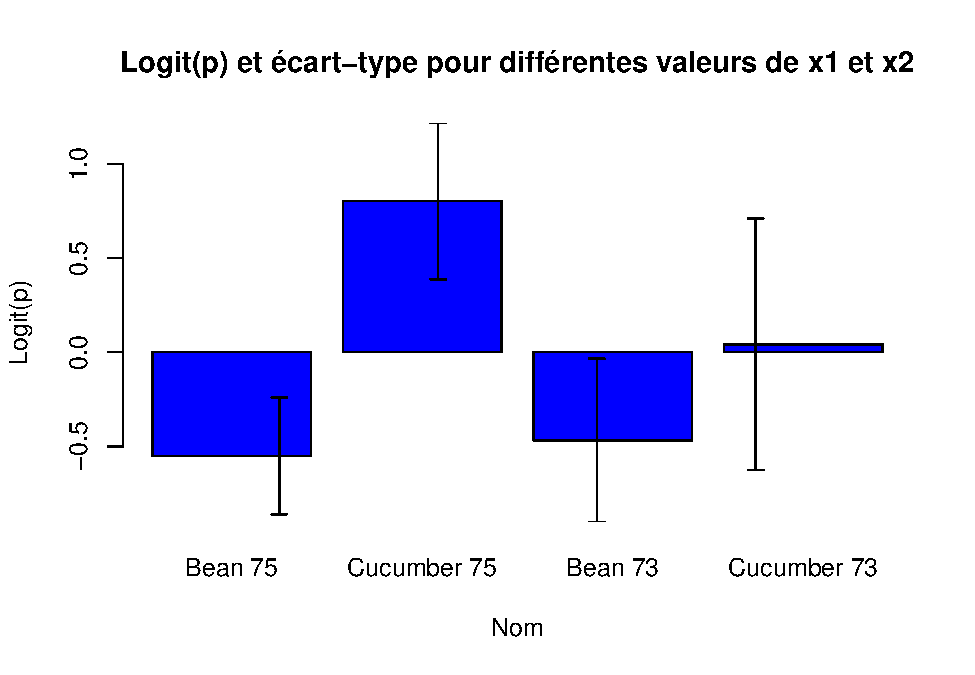
\includegraphics{projet1---rapport_files/figure-latex/unnamed-chunk-2-1} \end{center}

\begin{center}\includegraphics{projet1---rapport_files/figure-latex/unnamed-chunk-2-2} \end{center}

Les résultats obtenues sont cohérents avec l'objectif initial visé dans
l'énoncé. Les valeurs sont distribuées autour des moyennes attendues et
les écart-types sont également en accord avec les attentes, en observant
des variations inférieurs à 20 (sauf pour sigma)

\hypertarget{interpruxe9tation-des-ruxe9sultats}{%
\section{Interprétation des
résultats}\label{interpruxe9tation-des-ruxe9sultats}}

On va maintenant essayer de voir l'impact de x1 et x2 sur logit(p). Pour
cela, on réutilise les moyennes des variables aléatoires que l'on a
calculé avant.

\begin{table}[h]
\centering
\small
\begin{tabular}{|c|c|c|c|c|}
\hline
\textbf{Nom} & \textbf{x1} & \textbf{x2} & \textbf{logit(p)} & \textbf{ecart-type}\\
\hline
Bean 75 & 0 & 0 & -0.5517254 & 0.309775 \\
Cucumber 75 & 0 & 1 & 0.8027722 & 0.4157986 \\
Bean 73 & 1 & 0 & -0.4682697 & 0.4345104 \\
Cucumber 73 & 1 & 1 & 0.04229868 & 0.6678286 \\
\hline
\end{tabular}
\caption{Logit(p) pour différentes valeurs de x1 et x2}
\label{tab:tableau_combine}
\end{table}

\begin{center}\includegraphics{projet1---rapport_files/figure-latex/unnamed-chunk-3-1} \end{center}

On voit que le cucumber de l'aegyptiao 75 est celle qui a le plus de
chance de germer. C'est notamment plus élévé que pour l'autre type de
graine l'aegyptiao 73 avec la même racine (cucumber). Pour la racine
bean, on a mons de chance de germer que pour cucumber et il a très peu
de différences selon le type de graine(aegyptiao 75 ou aegyptiao 73).
\textgreater\textgreater\textgreater\textgreater\textgreater\textgreater\textgreater{}
b3fffae2b0c074065df4784c64dcb82510acce57

\end{document}
